\documentclass[10pt, varwidth=25cm]{standalone}

% For large-sized journals the figures should be 84 mm (for double-column text areas), 
% or 174 mm (for single-column text areas) wide and not higher than 234 mm. SAMO


\usepackage[utf8]{inputenc}
\usepackage{bm} % bold math letter
\usepackage{amsmath}
\usepackage{amsfonts}
\usepackage{stanli} % Structure Analisys tikz package
\usepackage{structmech}
\usepackage{siunitx}

% Tikz settings
\usepackage{pgfplots}
\usepackage{tikz}
\usetikzlibrary{decorations.pathreplacing,spy}
\usetikzlibrary{fit}
\usetikzlibrary{shapes.geometric}
\usetikzlibrary{shapes.arrows}
\usetikzlibrary{positioning}
\usetikzlibrary{decorations.pathreplacing,spy}
\usetikzlibrary{arrows.meta}

\pgfdeclarelayer{background}
\pgfsetlayers{background, main}
\pgfplotsset{compat=1.18}

\tikzstyle{decision} = [diamond, aspect=1.8, text centered, fill=white, draw=black, thick]
\tikzstyle{block} = [rectangle, draw=black, thick, fill=white, text centered, rounded corners, minimum height=2em]

\pgfplotsset{
    colormap={coolwarm}{
        rgb255(0cm)=(58,76,192);
        rgb255(1cm)=(64,84,199);
        rgb255(2cm)=(70,93,207);
        rgb255(3cm)=(76,102,214);
        rgb255(4cm)=(82,110,220);
        rgb255(5cm)=(90,120,227);
        rgb255(6cm)=(96,128,232);
        rgb255(7cm)=(103,136,237);
        rgb255(8cm)=(109,144,241);
        rgb255(9cm)=(117,152,246);
        rgb255(10cm)=(124,160,249);
        rgb255(11cm)=(131,166,251);
        rgb255(12cm)=(138,173,253);
        rgb255(13cm)=(145,179,254);
        rgb255(14cm)=(153,186,254);
        rgb255(15cm)=(160,191,254);
        rgb255(16cm)=(167,196,253);
        rgb255(17cm)=(174,201,252);
        rgb255(18cm)=(182,206,249);
        rgb255(19cm)=(188,209,246);
        rgb255(20cm)=(194,212,243);
        rgb255(21cm)=(200,215,239);
        rgb255(22cm)=(206,217,235);
        rgb255(23cm)=(213,219,229);
        rgb255(24cm)=(218,220,223);
        rgb255(25cm)=(223,219,217);
        rgb255(26cm)=(228,216,209);
        rgb255(27cm)=(233,212,201);
        rgb255(28cm)=(237,208,193);
        rgb255(29cm)=(240,204,185);
        rgb255(30cm)=(242,199,178);
        rgb255(31cm)=(244,194,170);
        rgb255(32cm)=(246,187,160);
        rgb255(33cm)=(247,181,152);
        rgb255(34cm)=(247,174,145);
        rgb255(35cm)=(246,167,137);
        rgb255(36cm)=(245,158,127);
        rgb255(37cm)=(243,150,120);
        rgb255(38cm)=(241,142,112);
        rgb255(39cm)=(238,134,105);
        rgb255(40cm)=(234,125,97);
        rgb255(41cm)=(230,114,89);
        rgb255(42cm)=(225,104,82);
        rgb255(43cm)=(220,94,75);
        rgb255(44cm)=(215,84,68);
        rgb255(45cm)=(207,70,61);
        rgb255(46cm)=(201,59,55);
        rgb255(47cm)=(194,45,49);
        rgb255(48cm)=(187,26,43);
        rgb255(49cm)=(179,3,38);
        },
        colormap name=coolwarm, 
        }

        \pgfplotsset{
    colormap={coolwarm_r}{
        rgb255(27cm)=(233,212,201);
        rgb255(28cm)=(237,208,193);
        rgb255(29cm)=(240,204,185);
        rgb255(30cm)=(242,199,178);
        rgb255(31cm)=(244,194,170);
        rgb255(32cm)=(246,187,160);
        rgb255(33cm)=(247,181,152);
        rgb255(34cm)=(247,174,145);
        rgb255(35cm)=(246,167,137);
        rgb255(36cm)=(245,158,127);
        rgb255(37cm)=(243,150,120);
        rgb255(38cm)=(241,142,112);
        rgb255(39cm)=(238,134,105);
        rgb255(40cm)=(234,125,97);
        rgb255(41cm)=(230,114,89);
        rgb255(42cm)=(225,104,82);
        rgb255(43cm)=(220,94,75);
        rgb255(44cm)=(215,84,68);
        rgb255(45cm)=(207,70,61);
        rgb255(46cm)=(201,59,55);
        rgb255(47cm)=(194,45,49);
        rgb255(48cm)=(187,26,43);
        rgb255(49cm)=(179,3,38);
        }
        }

\pgfplotsset{
    colormap={coolwarm_b}{
        rgb255(0cm)=(58,76,192);
        rgb255(1cm)=(64,84,199);
        rgb255(2cm)=(70,93,207);
        rgb255(3cm)=(76,102,214);
        rgb255(4cm)=(82,110,220);
        rgb255(5cm)=(90,120,227);
        rgb255(6cm)=(96,128,232);
        rgb255(7cm)=(103,136,237);
        rgb255(8cm)=(109,144,241);
        rgb255(9cm)=(117,152,246);
        rgb255(10cm)=(124,160,249);
        rgb255(11cm)=(131,166,251);
        rgb255(12cm)=(138,173,253);
        rgb255(13cm)=(145,179,254);
        rgb255(14cm)=(153,186,254);
        rgb255(15cm)=(160,191,254);
        rgb255(16cm)=(167,196,253);
        rgb255(17cm)=(174,201,252);
        rgb255(18cm)=(182,206,249);
        rgb255(19cm)=(188,209,246);
        rgb255(20cm)=(194,212,243);
        rgb255(21cm)=(200,215,239);
        rgb255(22cm)=(206,217,235);
        rgb255(23cm)=(213,219,229);
        rgb255(24cm)=(218,220,223);
        rgb255(25cm)=(223,219,217);
        }
        }
%-----------------------------
%- CUSTOM COLORS
%-----------------------------
\definecolor{accent_b_1}{RGB}{58,76,192}
\definecolor{accent_b_2}{RGB}{103,136,237}
\definecolor{accent_b_3}{RGB}{153,186,254}
\definecolor{accent_b_4}{RGB}{200,215,239}

\definecolor{accent_r_1}{RGB}{179,3,38}
\definecolor{accent_r_2}{RGB}{225,104,82}
\definecolor{accent_r_3}{RGB}{246,167,137}
\definecolor{accent_r_4}{RGB}{237,208,193}

\definecolor{axis_gray}{RGB}{120,120,120}
\definecolor{legend_gray}{RGB}{204,204,204}

%-----------------------------
%- CUSTOM NODES
%-----------------------------
\tikzstyle{point} = [circle,fill=white,draw,inner sep=0pt,minimum size=4pt]
\tikzstyle{forces} = [draw=accent_r_1,-stealth,very thick]
\tikzstyle{lab} = [align=center, fill=white,rounded corners=2pt, inner sep=1pt, font=\footnotesize]
\tikzstyle{arrow_reference} = [-{Triangle[open,length=2.8mm]}, line width=1pt]
%-----------------------------
%- MACROS
%-----------------------------
% Circled letters
\makeatletter
\usetikzlibrary{calc}
\newcommand*\circled[1]{\tikz[baseline=(char.base)]{
    \node[shape=circle, draw, inner sep=0pt, 
        minimum height={\f@size*1.4},] (char) {\vphantom{WAH1g}#1};}}
\makeatother


\newcommand{\norm}[1]{\lVert#1\rVert}
\newcommand{\vect}[1]{\bm{#1}}
\newcommand{\matr}[1]{\bm{#1}}

%-----------------------------
%- STYLE
%-----------------------------

% plot axis styles
\pgfplotsset{general2D/.style={ 
    footnotesize,
    scale only axis,
    axis x line=middle, 
    axis y line=middle, 
    xlabel={$x$}, ylabel={$y$}, 
    axis equal, 
    axis line style={-stealth,semithick},
    } 
}

\pgfplotsset{general3D/.style={ 
    scale only axis, 
    axis line style={-stealth,semithick},
    } 
}

\pgfplotsset{curves/.style={ 
        footnotesize,
        scale only axis, 
        xtick pos=left,
        ytick pos=left,
        axis x line*=bottom, % asterisk = no arrow
        axis y line*=left,
        clip=false,
        enlarge x limits={abs=0.15cm,lower},
        enlarge y limits={abs=0.15cm,lower},
        axis line style={thick, axis_gray, shorten <=0.136cm},
        every axis label/.append style ={axis_gray},
        every tick label/.append style ={axis_gray},
        every x tick/.style={color=axis_gray, thick},
        every y tick/.style={color=axis_gray, thick},
        tick align=outside,
        xlabel near ticks,
        ylabel near ticks,
        legend style={draw=none, font=\scriptsize},
        /pgf/number format/.cd,
        1000 sep={}
    } 
}

\pgfplotsset{curves_left/.style={ 
        scale only axis, 
        xtick pos=left,
        ytick pos=left,
        axis x line*=bottom, % asterisk = no arrow
        axis y line*=left,
        clip=false,
        tick label style={font=\scriptsize},
        every axis label/.append style ={axis_gray, font=\scriptsize},
        every tick label/.append style ={axis_gray},
        every x tick/.style={color=axis_gray, thick},
        every y tick/.style={color=axis_gray, thick},
        enlarge x limits={abs=0.15cm},
        enlarge y limits={abs=0.15cm},
        axis line style={axis_gray,thick, shorten <=0.136cm, shorten >= 0.136cm},
        tick align=outside,
        xlabel near ticks,
        ylabel near ticks,
        legend style={draw=none, font=\scriptsize\color{axis_gray}},
        /pgf/number format/.cd,
        1000 sep={}
    } 
}

\pgfplotsset{curves_right/.style={ 
        scale only axis, 
        xtick pos=left,
        ytick pos=right,
        axis y line*=right,
        x axis line style={draw=none},
        x tick style={draw=none},
        ytick pos=right,
        axis x line*=bottom, % asterisk = no arrow
        axis y line*=left,
        clip=false,
        tick label style={font=\scriptsize},
        every axis label/.append style ={axis_gray, font=\scriptsize},
        every tick label/.append style ={axis_gray},
        every y tick/.style={color=axis_gray, thick},
        enlarge x limits={abs=0.15cm},
        enlarge y limits={abs=0.15cm},
        axis line style={thick, shorten <=0.136cm, shorten >= 0.136cm},
        every y tick/.style={thick},
        tick align=outside,
        ylabel near ticks,
        legend style={draw=none, font=\scriptsize},
        /pgf/number format/.cd,
        1000 sep={}
    } 
}

\pgfplotsset{curves_3D/.style={ 
        footnotesize,
        scale only axis, 
        % xtick pos=left,
        % ytick pos=left,
        % ztick pos=left,
        axis x line*=bottom, % asterisk = no arrow
        axis y line*=left,
        axis z line*=left,
        clip=false,
        % enlarge x limits={abs=0.15cm,lower},
        % enlarge y limits={abs=0.15cm,lower},
        axis line style={thick, axis_gray, shorten <=0.136cm},
        every axis label/.append style ={axis_gray},
        every tick label/.append style ={axis_gray},
        every x tick/.style={color=axis_gray, thick},
        every y tick/.style={color=axis_gray, thick},
        every z tick/.style={color=axis_gray, thick},
        tick align=outside,
        % xlabel near ticks,
        % ylabel near ticks,
        legend style={draw=none, font=\scriptsize},
        /pgf/number format/.cd,
        1000 sep={},
        view={25}{40},
        colormap name=coolwarm,
    } 
}

\pgfplotsset{line_plot/.style={ 
            thick} 
}

\pgfplotsset{scatter_plot_smooth/.style={ 
    thick,
    mark size=1.5, 
    mark=*,
    mark options={solid}, 
    smooth }
}

\pgfplotsset{scatter_plot/.style={ 
    thick,
    mark size=1.5, 
    mark=*,
    mark options={solid}, 
    only marks} 
}

\pgfplotsset{scatter_plot_lin/.style={ 
    thick,
    mark size=1.5, 
    mark=*,
    mark options={solid},} 
}





\begin{document}

\begin{figure}
    \centering
    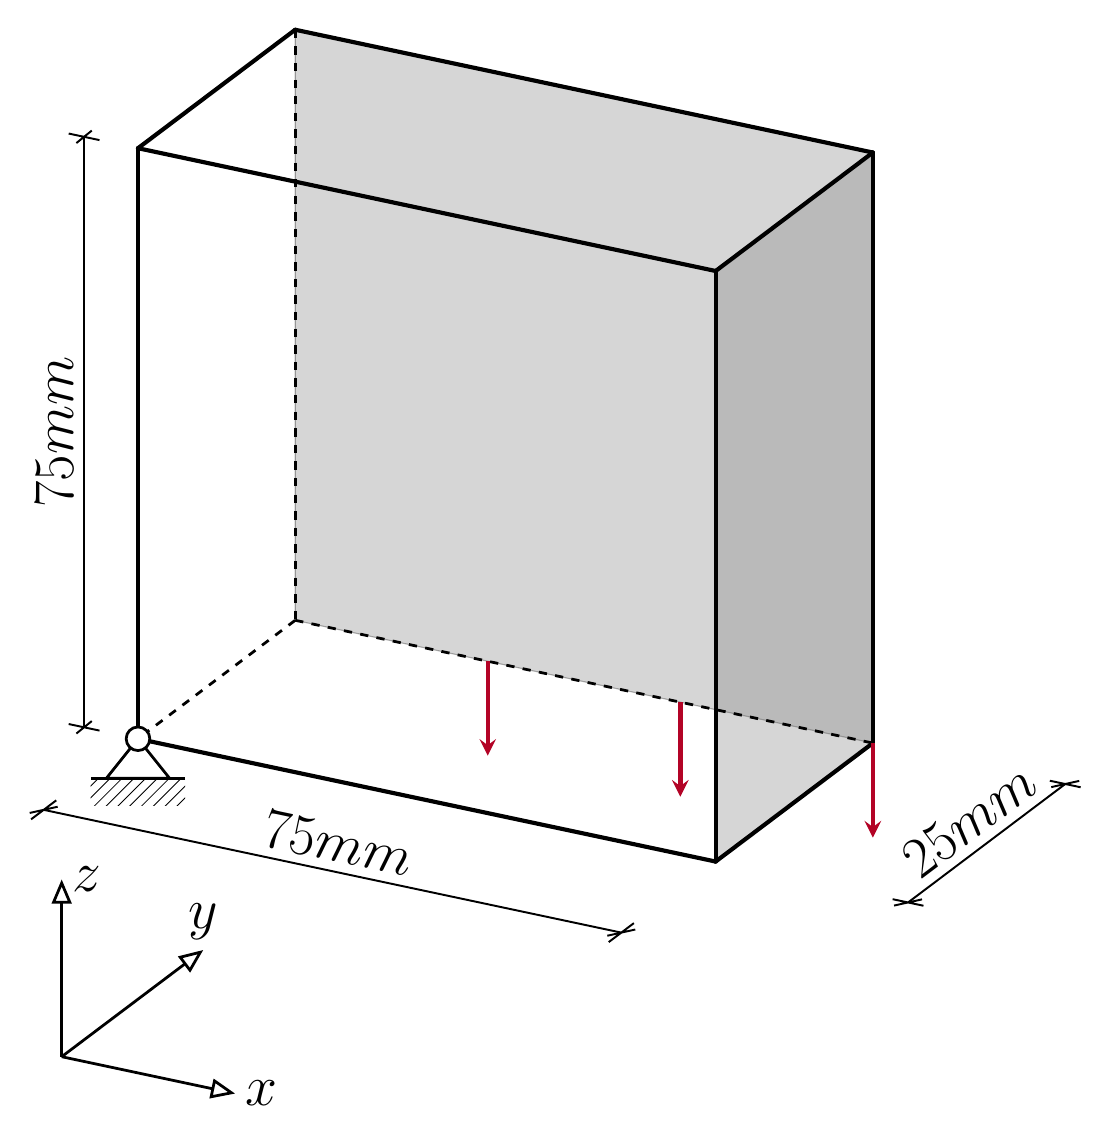
\begin{tikzpicture}[coords]
        % DIMENSIONS
        \def\x{7.5}
        \def\y{2.5}
        \def\z{7.5}
        \def\zz{2.5}
        \def\zzz{5}

        % CELLS
        \def\xcell{3}
        \def\ycell{1}
        \def\zcell{3}
        
        % POINTS
        \dpoint{a}{0}{0}{0};
        \dpoint{b}{0}{0}{\z};
        \dpoint{c}{0}{\y}{\z};
        \dpoint{d}{0}{\y}{0};
        \dpoint{e}{\x}{0}{0};
        \dpoint{f}{\x}{0}{\z};
        \dpoint{g}{\x}{\y}{\z};
        \dpoint{h}{\x}{\y}{0};
        
        \dpoint{i}{0}{0}{\zz};
        \dpoint{j}{\x}{0}{\zz};
        \dpoint{k}{\x}{\y}{\zz};
        \dpoint{l}{0}{0}{\zzz};
        \dpoint{m}{\x}{0}{\zzz};
        \dpoint{n}{\x}{\y}{\zzz};

        % % Draw the front face
        \draw[thin, fill=axis_gray,  opacity=0.3] (h) -- (d) -- (c) -- (g) -- cycle;
        
        % % Draw the back face
        \draw[thin, fill=axis_gray,  opacity=0.3] (e) -- (h) -- (g) -- (f) -- cycle;

        % % Draw the front face
        % \draw[thin, fill=accent_r_3,  opacity=0.3] (i) -- (j) -- (m) -- (l) -- cycle;
        
        % % Draw the back face
        % \draw[thin, fill=accent_r_3,  opacity=0.3] (j) -- (k) -- (n) -- (m) -- cycle;

        % % Draw the front face
        % \draw[thin, fill=accent_r_4,  opacity=0.3] (l) -- (m) -- (f) -- (b) -- cycle;
        % \draw[thin, fill=accent_r_4,  opacity=0.3] (m) -- (n) -- (g) -- (f) -- cycle;
        % \draw[thin, fill=accent_r_4,  opacity=0.3] (b) -- (f) -- (g) -- (c) -- cycle;



        % load points
        % \dpoint{l1}{\x/4}{\y-0.3}{\z};
        % \dpoint{l2}{\x/4}{0-0.3}{\z};
        % \dpoint{l2-2}{\x/4}{0}{\z-0.4};
        % \dpoint{l3}{\x/4}{0}{-0.4};

        % \dpoint{l4}{\x/2}{\y-0.3}{\z};
        % \dpoint{l5}{\x/2}{0-0.3}{\z};
        % \dpoint{l5-2}{\x/2}{0}{\z-0.4};
        % \dpoint{l6}{\x/2}{0}{-0.4};

        % \dpoint{l7}{3*\x/4}{\y-0.3}{\z};
        % \dpoint{l8}{3*\x/4}{0-0.3}{\z};
        % \dpoint{l8-2}{3*\x/4}{0}{\z-0.4};
        % \dpoint{l9}{3*\x/4}{0}{-0.4};

        % xz plane
        % \foreach \zz in{1,...,\zcell}
        % {
        %     \draw[thin, black] (0,0,\zz/\zcell*\z) -- (\x,0,\zz/\zcell*\z);
        %     \draw[dashed, thin, black] (0,\y,\zz/\zcell*\z) -- (\x,\y,\zz/\zcell*\z);
        % }
        % \foreach \xx in{1,...,\xcell}
        % {
        %     \draw[thin, black] (\xx/\xcell*\x,0,0) -- (\xx/\xcell*\x,0,\z);
        %     \draw[dashed, thin, black] (\xx/\xcell*\x,\y,0) -- (\xx/\xcell*\x,\y,\z);
        % }
        % % xy plane
        % \foreach \yy in{1,...,\ycell}
        % {
        %     \draw[thin, black] (0,\yy/\ycell*\y,\z) -- (\x,\yy/\ycell*\y,\z);
        %     \draw[dashed, thin, black] (0,\yy/\ycell*\y,0) -- (\x,\yy/\ycell*\y,0);
        % }
        % \foreach \xx in{1,...,\xcell}
        % {
        %     \draw[thin, black] (\xx/\xcell*\x,\y,\z) -- (\xx/\xcell*\x,0,\z);
        %     \draw[dashed, thin, black] (\xx/\xcell*\x,\y,0) -- (\xx/\xcell*\x,0,0);
        % }
        % % yz plane
        % \foreach \yy in{1,...,\ycell}
        % {
        %     \draw[thin, black] (\x,\yy/\ycell*\y,\z) -- (\x,\yy/\ycell*\y,0);
        %     \draw[dashed, thin, black] (0,\yy/\ycell*\y,\z) -- (0,\yy/\ycell*\y,0);
        % }
        % \foreach \zz in{1,...,\zcell}
        % {
        %     \draw[thin, black] (\x,0,\zz/\zcell*\z) -- (\x,\y,\zz/\zcell*\z);
        %     \draw[dashed, thin, black] (0,0,\zz/\zcell*\z) -- (0,\y,\zz/\zcell*\z);
        % }
        % \foreach \xa [count=\xi] in {0,2.5,5,7.5}
        %     \foreach \ya [count=\yi] in {0,2.5}  
        %         \foreach \za [count=\zi] in {0,2.5,5,7.5}
        %             \foreach \xx [count=\xxi] in {0,2.5,5,7.5}
        %                 \foreach \yy [count=\yyi] in {0,2.5}  
        %                     \foreach \zz [count=\zzi] in {0,2.5,5,7.5}  
        %                         \draw[accent_b_3, thin] (\xa, \ya, \za) -- (\xx, \yy, \zz);


        %     \draw[accent_b_3, thin] (0,0,0) -- (2,2,2);

        % BEAMS
        \dbeam{2}{a}{b}
        \dbeam{2}{b}{c}
        \dbeam{3}{c}{d}
        \dbeam{3}{d}{a}
        \dbeam{2}{a}{e}
        \dbeam{2}{b}{f}
        \dbeam{2}{c}{g}
        \dbeam{3}{d}{h}
        \dbeam{2}{e}{f}
        \dbeam{2}{f}{g}
        \dbeam{2}{g}{h}
        \dbeam{2}{h}{e}

        % MESH
        %\draw[help lines, step =.3] ( 0 , 0) grid (\x, \y);
        %\draw[help lines, xstep =1*\scalingValueCell, ystep = 0.2*\scalingValueCell, yslant=-0.21] (b) grid (e);

        
        % % QUOTES
        \ddimensioning{xy}{a}{e}{-1.5}[\huge $75 mm$ ];
        \ddimensioning{zx}{a}{b}{-.7}[\huge $75 mm$ ];
        \ddimensioning{yx}{e}{h}{7.5 + 2.5}[\huge $25 mm$ ];

        % BC
        \support{1}{a};
        % \support{1}{d};
        % \support{1}{e};
        % \support{1}{h};
        \hinge{1}{a}
        % \hinge{1}{d}
        % \hinge{1}{e}
        % \hinge{1}{h}


        % LOADS  
        \foreach \xx in{1,...,3}
        {
            \draw[forces, accent_r_1, ultra thick] (\xx*2.5,2.5,0) -- (\xx*2.5,2.5,0-1.2);
        }

        % \node at (8.5,0,1.25+2.5+0.5) {\large symm.};


        \dscaling{3}{1.5};
        \setaxis{3}[\huge$x$][\huge$y$][\huge$z$][$a$][$b$][$c$]
        \daxis{1}{3.5,-5.5 ,0}[right][above][right];
    \end{tikzpicture} 
\end{figure}
\end{document}